\documentclass{article}
\usepackage[english]{babel}
\usepackage[utf8]{inputenc}
\usepackage{fancyhdr}
\usepackage{amsmath}
\usepackage{amsfonts}
\usepackage{listings}
\usepackage{color}
\usepackage[final]{pdfpages}
\newcommand{\minus}{\scalebox{0.75}[1.0]{$-$}}

\usepackage{hyperref}
\hypersetup{
	colorlinks=true,
	linkcolor=blue,
	filecolor=magenta,      
	urlcolor=cyan,
}

\lstset{frame=tb,
	language=Java,
	aboveskip=3mm,
	belowskip=3mm,
	showstringspaces=false,
	columns=flexible,
	basicstyle={\small\ttfamily},
	numbers=none,
	numberstyle=\tiny\color{gray},
	keywordstyle=\color{blue},
	commentstyle=\color{dkgreen},
	stringstyle=\color{mauve},
	breaklines=true,
	breakatwhitespace=true,
	tabsize=3
}


\begin{document}
	
	\pagestyle{fancy}
	\fancyhf{}
	
	\title{DS-GA-1003: Spring 2017 \\ 
		Machine learning and Computational Statistics \\ 
		Project Proposal}
	\date{\today}
	\author{Siyang Sun(ss9558), Xinsheng Zhang(xz1757), Zemin Yu(zy937)}
	\maketitle
	\section{Business Problem}
	Founded in 2008, Airbnb keeps changing the way people live and travel. Not only do individuals share accommodations, but they also start to connect on unique stories and lifestyles through Airbnb, which has become a symbol of the sharing economy. With its rapid expansion in the whole world, Airbnb has already advertised over 3,000,000 lodging listings in more than 65,000 cities and 191 countries up till 2017. As students at New York University (NYU), we always love to explore the city we live in. In this project, we focus on Airbnb listings in New York City (NYC), a cosmopolitan and worldwide travel destination. We believe Airbnb could give us a distinct insight into characteristics of NYC neighborhoods.
	
	We would like to propose a model to predict appropriate prices for Airbnb listings in NYC. Particularly, we are interested in studying how these features would help Airbnb provide an internal tool to assist hosts in determining reasonable prices. If time is allowed, we would also like to apply natural language processing (NLP) techniques on housing reviews, and integrate them into our predictive model.
	
	\section{Data}
	We will use datasets provided by \href{http://insideairbnb.com/get-the-data.html}{Inside Airbnb} where the data is sourced from publicly available information from the Airbnb site. For this project, we will concentrate on NYC data, which is compiled on December 3rd, 2016.
	
	The data is separated into two datasets. We will mainly focus on \textit{listing} dataset, which records detailed listing information in NYC. It contains 40,227 unique listings and 95 features in total. The features are roughly divided into the following groups.
	\begin{itemize}
		\item listing: name, space, description, accommodates, etc.
		\item host: about host, response rate, verification, etc.
		\item location: latitude, longitude, zip code, borough, etc.
		\item availability: maximum nights, security deposit, etc.
		\item review: review scores, reviews per month, etc.
		\item \texttt{price}
	\end{itemize}
	
	Specifically, our target variable \texttt{price} is continuous. From the summary table and the truncated histogram graph below, the variable has a heavy right tail, which indicates lots of outliers. 
	
	\begin{table}[h!]
		\centering
		\begin{tabular}{|c|c|c|c|c|c|c|}
			\hline
			Mean   & SD     & Min & 25\% & 50\% & 75\% & Max  \\ \hline
			147.48 & 210.22 & 10  & 70   & 109  & 175  & 9999 \\ \hline
		\end{tabular}
		\caption{\texttt{price} summary}
	\end{table}
	\begin{figure}[h!]
		\centering
		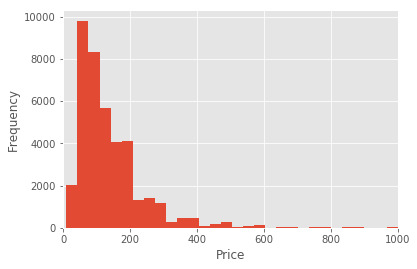
\includegraphics[width=10cm]{figure1}
		\caption{\texttt{price} distribution (truncated)}
	\end{figure}
	
	Optionally, the other \textit{review} dataset collects detailed reviews for each listing. It contains a total of 614,127 reviews for 31,150 distinct listings.
	
	Upon our initial data exploration, we will face these following technical difficulties in our data mining problem:
	\begin{itemize}
		\item Most of the columns (53) contains null value, and 9 of them has more than $50\%$ null. We need to figure out a reasonable way to clean null columns and impute null values.
		\item Lots of columns (63) are natural language, which requires NLP techniques to extract features. In addition, there are entries recorded in non-English language. 
		\item Some features are categorical with a large number of unique values (for example, neighborhoods). We need to one-hot such variable, and thus are also likely to introduce too many dimensions. 
		\item Not all the features are useful to predict the house price. Feature selection and feature engineering are required to select best subset to maximize the information gain. 
	\end{itemize}
	
	\section{Machine Learning Formulation}
	Some baseline algorithms to predict listing price include but not limited to linear regression (with regularization), linear decision tree and random forest based on a basic feature set. Since there are several options, we plan to accomplish some preliminary model performance evaluation before our second meeting with the adviser.
	
	\section{Timeline}
	\begin{itemize}
		\item \textbf{March 23: Project Proposal Due}
		\item March 24 - March 31: Data inspection
		\begin{itemize}
			\item Data cleaning and missing value imputation
			\item Data Visualization
			\item Descriptive statistical analysis
		\end{itemize}
		\item April 1 - April 18: Feature engineering; Baseline evaluation
		\item \textbf{April 19: Second meeting with advisers}
		\item April 20 - May 2: Model selection and evaluation; Performance and Error Analysis
		\item \textbf{May 3: Third meeting with advisers}
		\item \textbf{May 9: Project Poster Session}
		\item \textbf{May 12: Final Project Report Due}
	\end{itemize}
\end{document}